\documentclass[10pt, conference, compsocconf]{IEEEtran}

\title{Mitigating Interest Flooding DDoS Attacks in Named Data Networking}%:\\ Cache/Content Poisoning}
\author{anonymous}

\usepackage{graphicx}
% \usepackage[colorlinks]{hyperref}
\usepackage[]{hyperref}
\usepackage{breakurl}
\usepackage{url}
\usepackage[nocompress]{cite}
% \usepackage{verbatim}
% \usepackage{algpseudocode}
\usepackage{algorithm}
\usepackage{algpseudocode}

\graphicspath{{figures/}}

\begin{document}
\maketitle

\begin{abstract}

Distributed Denial of Service attack is an ongoing problem in today's Internet. 
A newly proposed future Internet architecture, Named Data Networking (NDN), lets end users request desired data by sending Interest packets, and the network forwards data packets to end users upon request only. 
Thus, NDN can effectively defeat the existing DDoS attacks, however it can be subject to new types of DoS attacks, namely Interest packet flooding.  
In this paper we investigate effective solutions to mitigate Interest flooding attacks. 
We use simulations to evaluate the design and our results show that our proposed solution can respond to Interest flooding attacks quickly, and that the inherent flow-balance property of NDN (i.e., one Interest packet retrieves at most one Data packet) can be used as a basis for effective DDoS mitigation algorithms.

\end{abstract}

\begin{IEEEkeywords}
Information-Centric Networks, Named-data Networking, Denial-of-Service
\end{IEEEkeywords}

\section{Introduction}
\label{sec:intro}

% Introduction / Motivation
% Brief introduction about attacks in NDN
% Contributions of the paper

% Introduction to the problem: ndn, solves many problems, but has potential to introduce new problems.
% in this paer we are studing a number of remedies to Interest floodig attack, as well as trying to doscover ptential of tjese dolutions and their shortcomings

% Structure. Hopefully around three paragraps. 
% - what is happening with ndn and what is interest floodog
% - what are the general approaches we are taking, ranging from naïve to more intelligent
% - basic summary of the results

% move disclaimer from section 3 to the intro.

The Internet is a unique global success story that earmarked the information age. However, the design that fostered its success and wide-adaptation over the last three decades is now aged and limited in accommodating the changing demands of today's users. Named Data Networking (NDN)~\cite{ndn-conext, ndn-tr} is an active research effort that aims to move the Internet into the future with a new, content-centric design that is capable of efficient content distribution and seamless mobility support. 

In contrast to today's Internet, a key goal of the NDN project is ``security by design". In fact, it goes a long way by guaranteeing the integrity and provenance of every data packet with digital signatures and protecting user-privacy with no source addresses carried in packets. However one big question that is yet to be answered is: How does the current NDN design fare in terms of its resilience against denial of service attacks? Especially since various forms of distributed denial of service (DDoS) attacks pose a significant threat to the existing Internet infrastructure~\cite{arbor-report}, it is crucial that any design aiming to replace it would be free of similar vulnerabilities.

NDN makes data the first-class network entity and eliminates host-based addressing. Instead of allowing end hosts to send packets
to a given IP address, NDN allows end hosts to request desired
data by sending Interest packets carrying application level
data names. Such a shift automatically eliminates several long
standing DDoS attacks, including direct flooding as well
as reflector attacks through source address spoofing~\cite{mirkovic2004taxonomy}.

However, since NDN allows any host to request any data, malicious users can attack the network by sending excessive number of data requests. Such requests are expressed by sending Interests packets and each Interest stores state and consumes resources at intermediate routers as it is routed through the network. Thus, excessive number of Interests can easily disrupt service by exhausting router memory. We coin in the term {\it Interest flooding} to refer to such attacks and
%One can also attack an NDN network by hijacking Interest packets and then injecting false data replies into the network.
this paper exclusively investigates the problem and the solution space for it. Our effort is an important first step towards a complete investigation of denial of service attacks in NDN. We show the devastating effect of Interest flooding on vanilla NDN and propose three algorithms that allow routers to exploit their state information to effectively thwart these attacks. Through extensive simulations on real network topologies,  we show how one of our mitigation methodologies effectively shuts down malicious users while allowing legitimate users to not experience any service degradation. 
%We use extensive simulations to show the devastating effect of Interest flooding on vanilla NDN and how a router can effectively exploit its state information to effectively mitigate them. 
 %(Section~\ref{sec:design}).
%We base our solutions on the following two insights.
%First, instead of creating state for all incoming Interests, an NDN router should only needs to accept enough Interest packets to fully utilize downstream link capacity.
%Second, because Data packets traverse the path taken by the Interests, an NDN router can observe whether an Interest retrieves Data (good %Interest) or not (bad Interest).
% Alex: Not sure whether it should be mentioned in intro or not.  If it should, then I don't really like it...
The rest of the paper is organized as follows: We give an overview of NDN architecture in Section~\ref{sec:ccn-intro} and explain interest flooding attacks in Section~\ref{sec:interest-flooding}. In Sections~\ref{sec:design},~\ref{sec:evaluation} and~\ref{sec:discussion}, we introduce techniques to mitigate these attacks, evaluate their effectiveness and discuss their limitations respectively. We summarize related work in Section~\ref{sec:related-work} and finalize the paper with conclusions and future work in Section~\ref{sec:conclusion}.

%We conduct simulation-based evaluations to quantify the effectiveness of our proposed attack mitigation algorithms %(Section~\ref{sec:evaluation}).
%% based on trivial small-scale and Internet-like larger-scale topologies.
%The results show a great potential of one of the designed algorithms (satisfaction-based pushback, Section~\ref{sec:dynamic limits}), where %the attack traffic can be effectively localized near the attacker himself.
%\todo{LZ: I did not modify this last paragraph; need to see the rest of the paper first.}



%%% Local Variables: 
%%% mode: latex
%%% TeX-master: "paper"
%%% End: 


\section{NDN Overview\label{ccn-intro}}
%Named Data Networking (NDN) is a network architecture which aims to replace IP architecture by replacing IP�s host-to-host data delivery model with pull-based information retrieval model. In IP in order to retrieve data, data consumer have to know endpoint location of the desired data, in NDN all they have to know is data name. Names are hierarchical (non-flat) application-defined string names that are used for forwarding, routing and caching. A canonical NDN name looks in a following way: /ndn/ucla/CSdept/faculty/Lixia/webpage.

In this section we briefly introduce NDN with a focus on its stateful forwarding plane (for more details refer to \cite{ndn-conext, ndn-tr, adaptive-forwarding}).
NDN is a receiver-driven, data-centric communication protocol.
All communication in NDN is performed using two distinct types of packets: \textit{Interest} and \textit{Data}. Both types of packets carry a \textit{name}, which uniquely identifies a piece of data that can be carried in one Data packet. Data names in NDN are hierarchically structured. A canonical NDN name looks in the following way: \ndnName{/ndn/ucla/CS/www/index.html}.

To retrieve Data, a consumer puts the name of the desired content into an Interest packet and sends it to the network.
Routers use this name to forward the Interest towards the Data producer, and the Data packet whose name matches the name in the Interest is returned to the consumer.  All Data packets carry a signature that binds the name to the Data.
An Interest is ``satisfied'' when a Data packet is received with matching data name.

Each NDN router maintains three major data structures:
\begin{itemize}
\item \textit{Pending Interest Table (PIT)} holds all ``not yet satisfied'' Interests that have been sent upstream towards data producers. Each entry in PIT contains a list of incoming, and outgoing, physical interfaces; the former enables multicast Data delivery, and the latter is needed when the same Interest is forwarded along multiple paths.
\item \textit{Forwarding Interest Base (FIB)} maps name prefixes to one or multiple physical network interfaces, defining allowed (multipath) directions where to forward Interests. 
% Having one-to-many relationship in this table allows multipath forwarding of Interests.}
\item \textit{Content Store (CS)} temporarily buffers Data packets that pass through this node, allowing fast Data retrieval by different consumers.
\end{itemize}

When a router receives an Interest packet, it first checks whether there is a matching Data in its CS.
If a match is found, the Data is sent back to the incoming interface of the Interest packet.
If not, the Interest name is checked against the entries in the PIT. 
If the name exists in the PIT already, then it can be either a duplicate Interest (i.e., its nonce is remembered in PIT entry) that should be dropped,
or an Interest from another consumer asking for the same Data which requires the incoming interface of this Interest to be added to the existing PIT entry (``collapsing'' the Interests).
If the name does not exist in the PIT, the Interest is added into the PIT and further forwarded to the interface chosen by the strategy module, which uses FIB as input for its decision.

When a Data packet is received, its name is used to look up the PIT.
If a matching PIT entry is found,
the router sends the Data packet to the interface(s) from which the Interest was received, caches the data in the CS, and removes the PIT entry.  Otherwise, the Data packet is unsolicited and discarded. 
Each Interest also has an associated lifetime; the PIT entry is removed when the lifetime expires.
The lifetime is specified by users, but it is ultimately a router's decision for how long it is actually willing to keep the PIT entry.  
For example, and we assume this in the rest of the paper, the maximum time any Interest is kept in PIT is one second.

%Every incoming Interest triggers a lookup in the Content Store and if the Data with matching data name have been found, it is sent back to the same physical interface from which the Interest has arrived. If CS lookup is unsuccessful, Interest must be sent further upstream and put in the PIT. However, all recurring Interests with the same prefix name are stacked together in the same PIT entry and are not sent to the upstream again until this PIT entry expires completely because of timeout. If Data returns from some upstream location it is replicated for each incoming physical interface stored in this PIT entry after that it is removed from PIT. In other words, multipath Data delivery is built-in in NDN. 


%\begin{figure}[htpb]
%  \centering
%  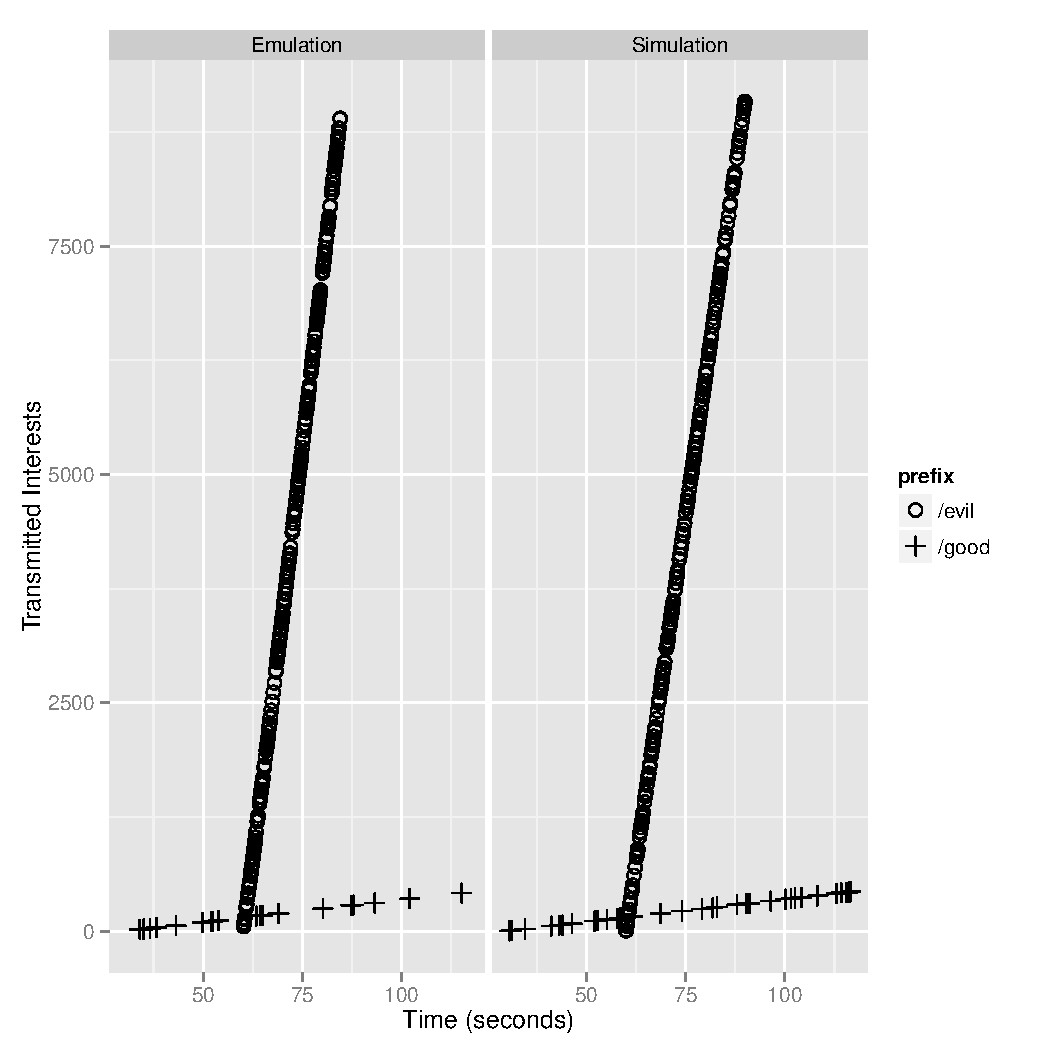
\includegraphics[scale=0.5]{figures/sim-emu-power.pdf}
%  \caption{Strength of Interest flooding attack}
%  \label{fig:simemupower}
%\end{figure}

%\begin{figure}[htpb]
%  \centering
%  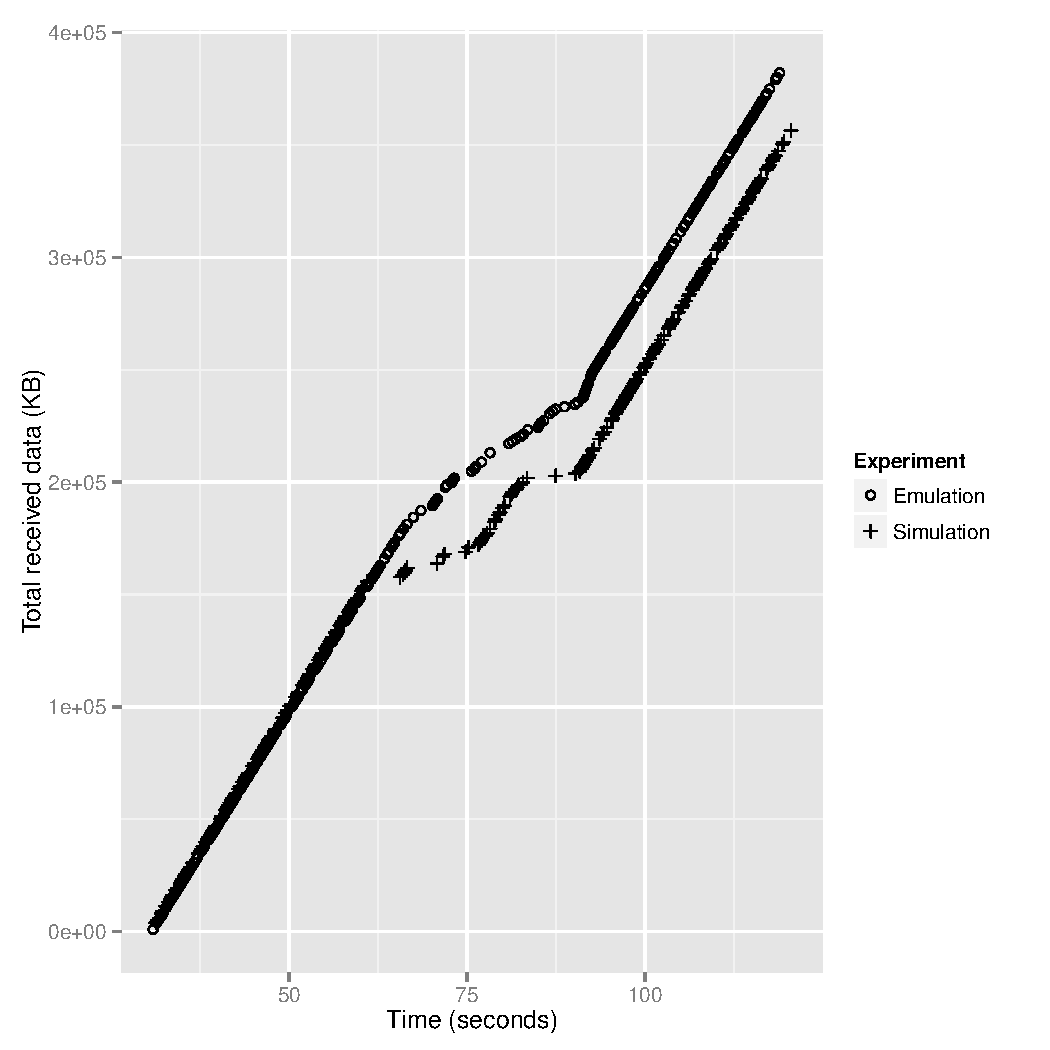
\includegraphics[scale=0.5]{figures/sim-emu-performance.pdf}
%  \caption{Data retrieval by legitimate clients}
%  \label{fig:simemuperf}
%\end{figure}


%%% Local Variables: 
%%% mode: latex
%%% TeX-master: "paper"
%%% End: 


\section{Interest Flooding in NDN}
\label{sec:interest flooding}

Any DoS attack aims to exhaust system resources. In the context of NDN by term "system" we understand two things: 1) every individual NDN router 2) a distributed system consisting of some collection of NDN routers. In a first case, every major data structure (FIB, CS, PIT) is a potential surface for denial of service attack. In a second case, we consider: 1) bandwidth between NDN routers 2) caching capabilities of NDN routers 3) packet processing capabilities of NDN routers.

Let's examine an individual NDN router first. Certainly, as any other piece of software each specific NDN implementation can have bugs and exploits e.g. buffer overflows leading to data corruption in cache, etc. In this paper we are assuming an idealized NDN implementation lacking any implementation bugs. 

In a general case, Forwarding Interest Base (FIB) is managed by routing protocol and if attackers have been able to get control over routing, they could advertise a huge number of FIB announcements that will fill up FIB table that may cause Interest processing delays and traffic redirection with amplification or black-holing.

Pending Interest Table (PIT) is used to keep per packet forwarding state in NDN and is critical for Data delivery. Though PIT table has an upper limit on its size, it doesn't prevent attacker from injecting a huge number of false Interest packets at a very high rate, which eventually will lead to a situation where the whole PIT table is full of false Interest packets and is not able to keep forwarding state of Interests coming from legitimate users. This attack may look similar to TCP SYN-flood attack and we call it Interest flooding. 

Content Store (CS) is an effective obstacle for several types of DDoS attacks. CS possesses two important characteristics: maximum size and replacement policy. However, by knowing replacement policy attacker can construct a specific traffic generator that is using weaknesses of a chosen replacement procedure that will lead to increased processing time, slower packet delivery and in some cases de facto a complete inability to cache legitimate data. 

An infrastructure consisting of NDN routers is vulnerable to the following types of attacks: 
\begin{enumerate}
\item Interest flooding. 
\item fkjgkfjgkfg
\end{enumerate} 
%\begin{figure}[htpb]
%  \centering
%  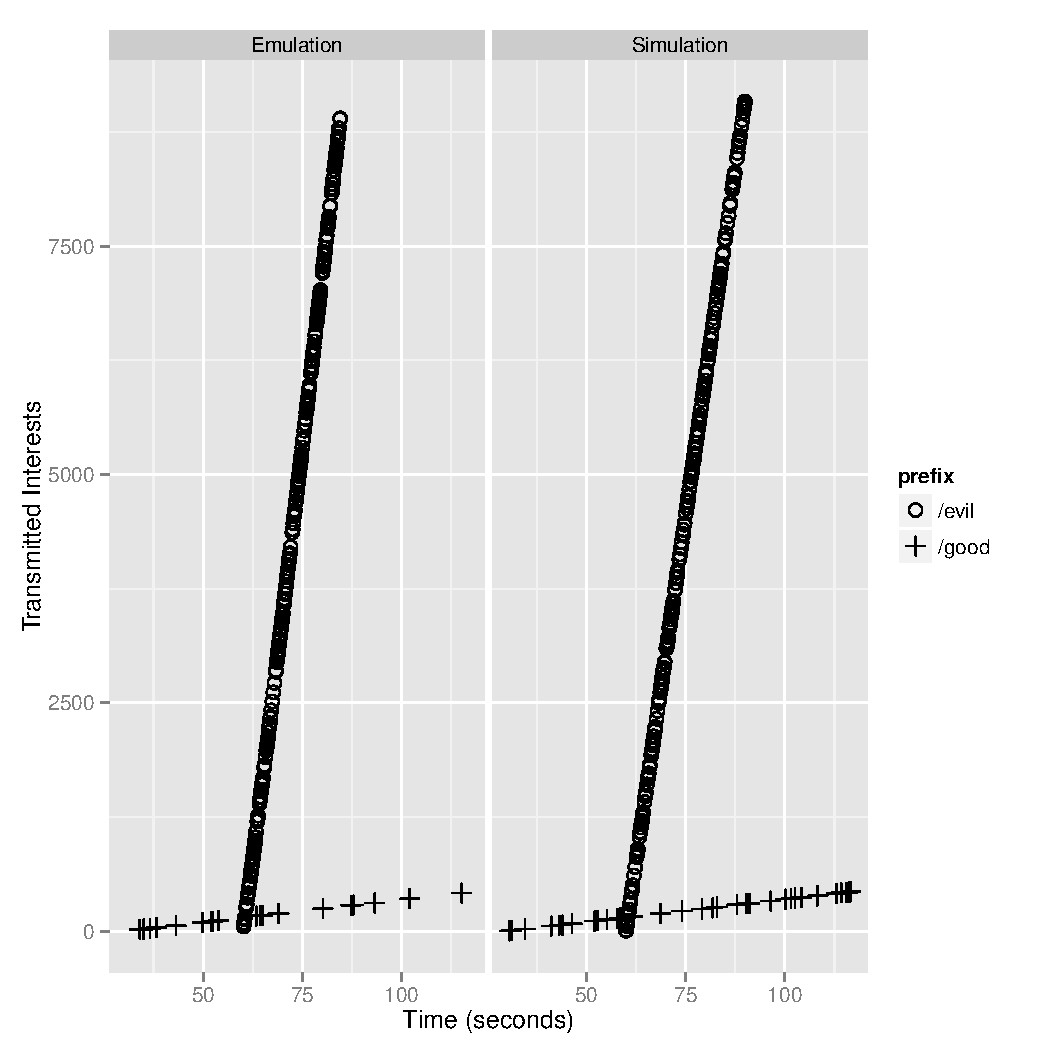
\includegraphics[scale=0.5]{figures/sim-emu-power.pdf}
%  \caption{Strength of Interest flooding attack}
%  \label{fig:simemupower}
%\end{figure}

%\begin{figure}[htpb]
%  \centering
%  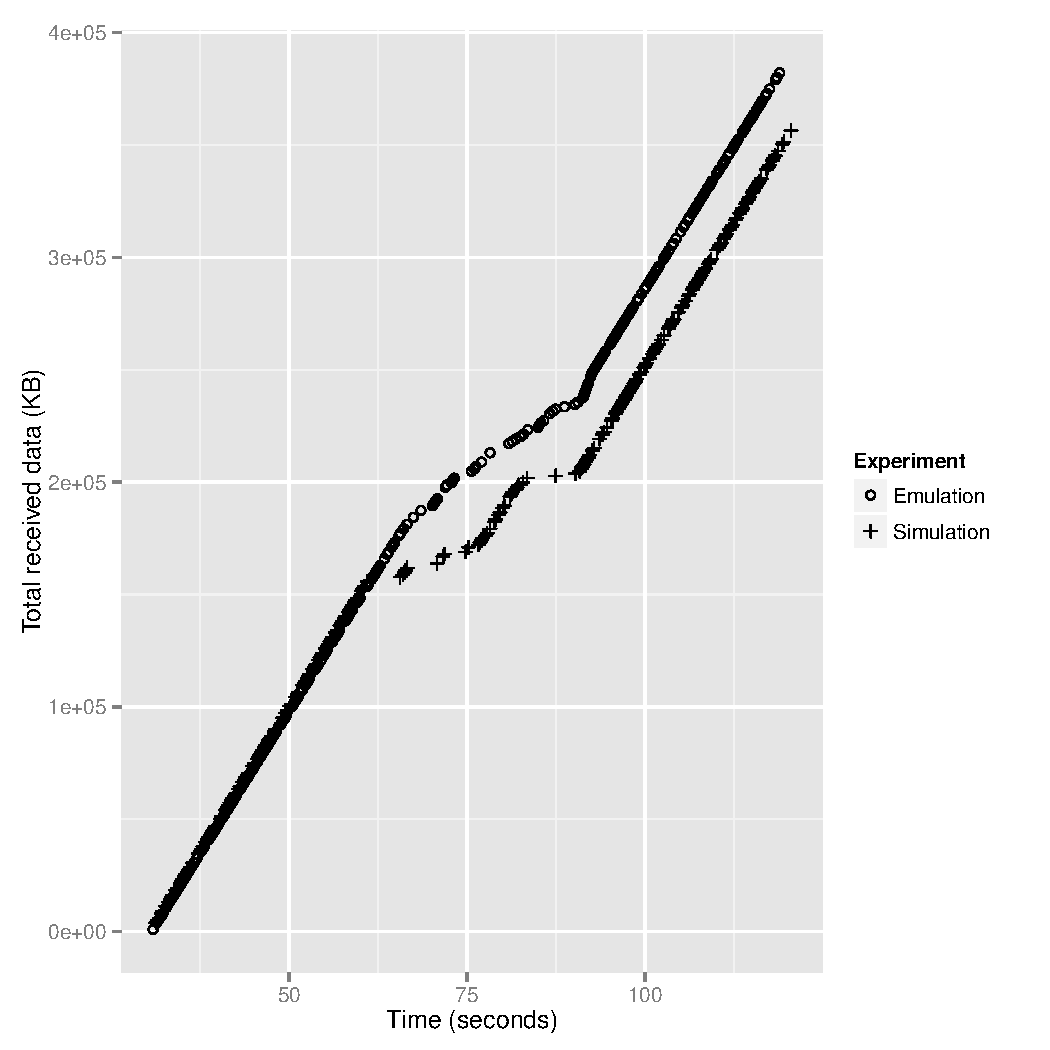
\includegraphics[scale=0.5]{figures/sim-emu-performance.pdf}
%  \caption{Data retrieval by legitimate clients}
%  \label{fig:simemuperf}
%\end{figure}


%%% Local Variables: 
%%% mode: latex
%%% TeX-master: "paper"
%%% End: 


\section{Interest flooding mitigation methods}
\label{sec:design}

% Points what should be here:
% - What can be done (in general) to mitigate flooding attack
% - Which building blocks NDN architecture gives to mitigate Interest flooding attacks: Interest limits, ability to measure Interest satisfaction performance (Interest satisfaction stats)
% - Methods to set these limits: static/dynamic
% - Methods how limits can be applied: best-effort (fifo), "fair" queuing, probabilistic
% - Reference to caching: we don't consider it here, but caching provides additional level of protection, especially for certain types of attacks

% Our definition of attack mitigation is that good clients are still able to access data on the producer.

In this section we present several algorithms to mitigate Interest flooding attacks in NDN.  Our mitigation strategies feature varying degrees of implementation complexity and effectiveness---the higher the implementation complexity, the more effective is the algorithm against Interest flooding attacks. We start by describing our simple strategies and use the insights and lessons learned from the deployment of these to inform and design more effective mitigation techniques that works well in various topologies.

%   - Naive approach to Interest Limits (that is called physical limits everywhere else)
%     Example how this can be implemented in a simple way
%     Baseline solution
%   - Interest limits with "fair" queuing
%     Improving problem of simple limits (no single face can dominate), but doesn't solve the proble

% - Attack mitigation
%   - Per-incoming interface Interest statistics

%   - Dynamic Interests limit adjustments

%   - Probabilistic Interest accept

%The fact that each Data packet takes the reverse path of the corresponding Interest packet allows intermediate routers to match a received Data packet to the corresponding Interest packet and %thus determine which Interest packets were satisfied. As we describe in the rest of this section,  NDN routers can exploit this information to make informed decisions on which Interest packets to %forward, how many Interest packets to forward, and thus effectively defend against DDoS attacks.

%Our methods to mitigate Interest flooding attack rely on the fundamental principle of the NDN architecture: the flow balance between Interest and Data packets: one Interest packet (the only communication initiator) can be satisfied with at most one Data packet.
%Because NDN is host-to-host architecture (as opposed to end-to-end in the current IP Internet), the flow balance principle allow any entity on the network, end-hosts and routers, control what and how much Data they want to receive.
%Therefore, any node can limit the number of forwarded Interests, effectively limiting the amount of the retrieved Data.
%At the same time, each forwarded Interest can be used to build up various data plane performance statistics, such as per-incoming interface ratios of satisfied Interests.

%\subsection{Na\"{i}ve attack mitigation}

%We start with a couple of naive strategies that can be used to migitate attacks in an NDN network and describe the pitfalls associated with these strategies.

% In a normal network operation, the size of Interests packets is supposed to be significantly smaller than the size of the requested Data.

% All communication in NDN network is host-to-host and receiver-driven.

An obvious and na\"ive solution to defend against Interest flooding attacks is to restrict the number of Interests that are forwarded in the network. To this end, we exploit a 
 fundamental principle of NDN architecture---flow balance between Interest and Data packets. The flow balance refers to the fact that one Interest can be satisfied by at most one Data packet. This principle allows intermediate routers to control the inbound data traffic by controlling the number of outstanding Interests in the network. 
One simple implementation technique  is for an NDN router to limit the number of forwarded Interests out of each interface based on the physical capacity of the corresponding interface. This technique is a slight modification of the well-known {\it Token Bucket} algorithm that is currently widely used in packet-switched networks. Analogous to the {\it Token Bucket} algorithm, NDN routers keep track of the amount of data requested that can fully utilize the downstream link (estimated from the number of forwarded Interests) and once the link capacity limit has been reached, they no longer forward new incoming Interests. Ideally, the number of tokens (the pending \emph{Interests Limit}) for each link will be proportional to the link's bandwidth-delay product (BDP)~\cite{tcp-survey}. We can formalize this value as follows:
% With the objective to request as many Data packets, as downstream link can pump through, we are getting the following equation for Interest limit:
%
\begin{equation}
\small \mathrm{Interest\ Limit} = Delay\ [s] \cdot \frac{\mathrm{Bandwidth\ [Bytes/s]}}{\mathrm{Data\ packet\ size\ [Bytes]}}
\end{equation}

In the above equation, \emph{Delay} is the expected time of Interest being satisfied and \emph{Data packet size} is the size of the returned Data packet.
Although both these values are not known a priori, it is not really necessary to use their exact values.
One can simply set the pending Interest limit based on the average values of round trip time and observed Data packet size, as the network buffers can smooth out most of the network fluctuations.

This {\it Token Bucket} approach might be exceptionally restrictive in forwarding Interests---not all Interests will result in a Data packet---and might result in underutilization of the network. However, the biggest drawback of this algorithm is the fact that it can nourish DDoS attacks. If a router has utilized all its tokens to forward malicious Interests, it can no longer forward incoming Interests from legitimate users till the pending malicious Interests start to expire. One way to get around the issue is to impose a per interface limit, so that malicious Interests are not allowed to entirely consume the limits of a specific interface. We describe this technique in greater detail below.

%That is, if it is known that the amount of already requested data ($=$~amount of forwarded Interests) can fully utilize the downstream link, an NDN node---either an end-user or an NDN router---has absolutely no point in forwarding new incoming Interests and creating corresponding PIT entries.
%For example, if a router A on Fig.~\ref{fig:flooding example} already forwarded 125 Interests requesting 1000-byte Data packets, any new incoming Interests can be almost safely dropped, provided the link capacity between A--B is 100~Mbps and delay is 10~ms.
%In other words, 125 Data packets returned by router B will fully utilize the link ($125 \times 1000 \mathrm{~bytes} \approx 10\mathrm{~ms} \times 100\mathrm{~Mbps}$) and any excess Data would be dropped.
%
%\subsubsection{\textbf{Interest limits (physical limits)}}
%\label{sec:physical limits}
%
%\subsection{Physical limits}
\label{sec:physical limits}

The requirement to send an Interest in order to receive Data packet, provides an NDN consumer a unique opportunity to request the right amount of Data.
Moreover, the same opportunity to control the amount of data flow is given not only to consumers, but all routers between consumer and producer (or nearby caches).  
In other words, every node, either a consumer or an intermediate router, is able to control how much data it wants to receive by limiting the number of forwarded Interests.

The limitation can implemented in a number of different ways, including leaky bucket scheduling and window-based flow control.
We decided to following TCP-like window-based flow control and applied the sliding window approach to implement Interest limits.

The size of the window defines how many Interests can be send out before Interests get satisfied or expired.
From the one hand, this size should be large enough to ``fill the pipe,'' meaning that a node needs to send enough Interests to receive Data at full capacity of the incoming link.
On the other hand, the window's size should not be too large to avoid excessive buffering and congestion of the Data packet.
Thus, the ideal size for such a window need to be defined proportional to link's bandwidth-delay product~\cite{tcp-survey}.
With the objective to request as many Data packets, as downstream link can pump through, we are getting the following equation for Interest limit:

\[
\mathrm{Interest\ Limit} = Delay\ [s] \cdot \frac{\mathrm{Bandwidth\ [Bytes/s]}}{\mathrm{Data\ packet\ size\ [Bytes]}}
\]

Note that the value of \textit{Delay} is not known a priory and varies between different Interest-Data flows.
However, we do not need to know the exact value of the delay and can set it as an average round trip delay among all flows (with a reasonable filtering of outliers).
This way, the statistical traffic multiplexing with link-level buffering will allow full utilization of the downstream link.
Exactly the same reasoning can be applied to the \textit{Data packet size} parameter, which can also be set to an average observed Data packet size.

Unlike rate-based approaches, window-based limiting does not require precise knowledge about the rate, as well does not need precise scheduling mechanisms.
Like in TCP, the window-based flow is self-clocking, easily adjusting itself to any traffic patterns.

%%% Local Variables: 
%%% mode: latex
%%% TeX-master: "../paper"
%%% End: 


%%%%%%%%%%%%%%%%%%%%%%%
%%%%%%%%%%%%%%%%%%%%%%%
%%%%%%%%%%%%%%%%%%%%%%%

\subsubsection{\textbf{Token bucket with per interface fairness}}
\label{sec:queuing}

To address the lack of fairness associated with the na\"ive {\it Token Bucket} approach, we modify it to ensure that the Interests forwarded by a router on each interface represent a fair mix of Interests received from neighboring nodes. For example, in Fig.~\ref{fig:flooding example} router A can ensure that the tokens associated with Interests sent out on interface {\texttt eth2}  are fairly distributed across incoming interfaces \texttt{eth0} and \texttt{eth1}. 
%Due to the expected small volume of Interests, we cannot merely rely on network buffers to perform statistical multiplexing of Interests, as they would almost never be %buffered.
%At the same time, until bag of tokens is not empty, there is no reason to delay Interest forwarding, as we do not known how many and from which interfaces Interests %will arrive in the future.
In order to achieve our goal of ensuring ``fair'' mixing of Interests from all neighboring nodes, 
%, we implement an additional features to support buffering of Interests, if they cannot be immediately forwarded. 
we extend the Pending Interest Table to support flagging of Interests that cannot be immediately forwarded and implement hierarchical queues for each interface (see Fig.~\ref{fig:queueing}). 
This mechanism is essentially a class based queuing~\cite{floyd1995link}, with classes for each outgoing and incoming interface.
%As an alternative to hierarchical queues, one can also use an approach based on virtual time. For details, please see ~\cite{zhang1990virtual}.
We note that unlike normal queuing, Interest queues do not actually store a packet, but merely a bi-directional pointer to the existing PIT entry.
Thus, a PIT entry can be quickly updated when the Interest is actually forwarded, and the element can be easily removed from the queue when the Interest expires.

%For the buffering part, we can reuse Pending Interest Table, with a small extension to support flagging of the Interests that cannot be forwarded immediately (see example on Fig.~\ref{fig:queueing}). 
%As for the mixing part, we need an additional fair queuing mechanism, which can be implemented in a form of hierarchical queues (on Fig.~\ref{fig:queueing})\footnote{This essentially is a class based queuing, with classes for each outgoing/incoming interface.} or using virtual time approach~\cite{zhang1990virtual}. 

\begin{figure}[thb]
  \centering
  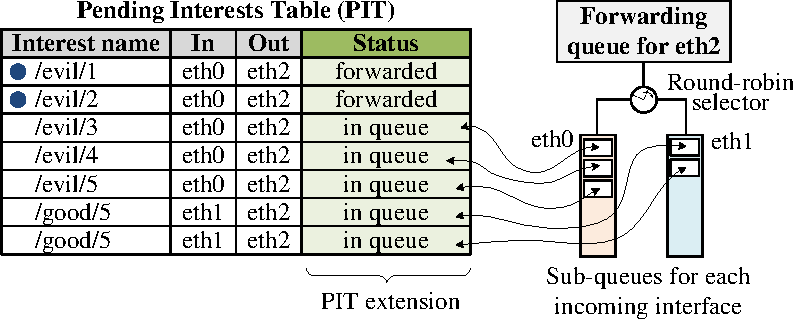
\includegraphics[scale=0.65]{queue}
  \vspace{-0.7cm}
  \caption{Interest queuing: if tokens are unavailable, the router creates a PIT entry, but instead of forwarding, it enqueues the Interest}
  \label{fig:queueing}
\end{figure}

We present a formalized description of this algorithm in Pseudocode~\ref{alg:queuing}. 
By setting appropriate queue sizes, we can control the amount of physical resources utilized at a router.
 % (such as memory and computation power). 
It is also important to set a sensible value for how long an Interest can be enqueued. 
If an Interest is enqueued for a long time, by the time it is dequeued and forwarded, the retrieved Data packet might be dropped at the downstream routers if their corresponding state expired. 
For our evaluations, we empirically chose to enqueue Interests up to 10\% of their original lifetime.
% We believe that implementing additional mechanisms on each pair of communicating routers to keep the Interests from getting stale would mitigate this issue, though the details are beyond the scope of this paper.
% Alex: I don't believe there is a need for separate discussion about "freshness", as we already introduced concept of lifetime
% {\color{red} \it Priya:  We need to  touch upon the Interest freshness issue in the NDN overview section; else we should get rid of this bit.}

%It should be noted that enqueued Interests should not be kept in the queue for a prolonged period of time.
%Otherwise, by the time the Interests reaches the Data, the state could have been long expired downstream, effectively making such an Interest useless.
%Additional mechanisms of pair-wise agreements between NDN routers and periodic Interest refresh can solve this particular problem, but it is out of the scope of the present paper.

%The algorithm extends the base Physical limits algorithm by enabling queuing when the bag of tokens is empty (lines 7--10), as well as by triggering an action (lines 16--21), when a token becomes available and enqueued Interest can be finally forwarded.
%At the same time, the algorithm limits number of Interests allowed in a queue, constraining memory usage increase by at most a constant factor, compared to the base Physical limits algorithm (i.e., memory attack on routers are still unfeasible). 


\floatname{algorithm}{\small Pseudocode}

%%%%%%%%%%%%%%%%%%%%%%%%%%%%%%
%%%%%%%%%%%%%%%%%%%%%%%%%%%%%%
%%%%%%%%%%%%%%%%%%%%%%%%%%%%%%

\begin{algorithm}[h]
\footnotesize
\caption{\small Token bucket with per interface fairness}
\label{alg:queuing}
\begin{algorithmic}[1]
\For{\textbf{each} interface \textbf{if}}
    \State{$L_{if} \leftarrow$ Interest Limit according to (1)}
    \State{$O_{if} \leftarrow 0$} \Comment{Outstanding Interests on interface \textbf{if}}
\EndFor

\vspace{0.1cm}

\Function{OutInterest}{Interest \textbf{i}, InInterface \textbf{in}, OutInterface \textbf{out}}
    \If{$L_{out} - O_{out} > 0$} \Comment{\textbf{out} is under limit cap}
        \State $O_{out} \leftarrow O_{out} + 1$  \Comment{``borrow'' a token from the bucket}
        \State add \textbf{out} to PIT entry and forward \textbf{i} to \textbf{out}
    \Else
        \State Queue $q \leftarrow out$.GetSubQueue($in$)
        \If{$Size(q) < L_{out}$}
           \State $q$.PushInterest($i$)
           \State add \textbf{out} to PIT entry, and link PIT entry with the queue
        \Else
           \State drop Interest
        \EndIf
    \EndIf
\EndFunction

\vspace{0.1cm}

\State{} \Comment{\textit{Whenever $L_{out} - O_{out}$ becomes larger than zero}}
\Function{TokenBecomesAvailable}{}
    \State Queue $q \leftarrow$ $out$.GetRoundRobinSubQueue 
    \State Interest $i \leftarrow$ $q$.PopInterest
    \State update PIT entry and Forward($i$, $out$)
\EndFunction

\vspace{0.1cm}

\Function{InData}{Data \textbf{d}}
   \State lookup PIT entry \textbf{p} for data \textbf{d}
   \For{\textbf{each} outgoing interface \textbf{out} in \textbf{p}}
        \State $O_{out} \leftarrow O_{out} - 1$ \Comment{``return'' token}
   \EndFor
\EndFunction

\vspace{0.1cm}

\Function{Timeout}{PIT entry $p$}
   \For{\textbf{each} outgoing interface \textbf{out} in \textbf{p}}
        \State $O_{out} \leftarrow O_{out} - 1$ \Comment{``return'' token}
   \EndFor
\EndFunction


\end{algorithmic}
\end{algorithm}


As we show in Section~\ref{sec:evaluation}, this algorithm provides partial relief from the Interest flooding attacks, allowing legitimate users to successfully fetch Data for 15--20\% of their expressed Interests. 
We note that while this algorithm might be reasonable for ensuring limited fairness in an NDN network, it is ineffective in protecting legitimate users from malicious ones. 
Attackers are able to successfully thwart access to content for legitimate users by sending a relatively modest volume of malicious Interests.


%At the same time, the Physical limits with or without fair queueing allows attackers to send a relatively small volume of Interests in order to significantly impact service for the legitimate users.
%Therefore, to successfully solve the problem, we need a fundamentally different, more intelligent approach, allowing localization of the attack traffic as close as possible to the attack origin.


%%%%%%%%%%%%%%%%%%%%%%%
%%%%%%%%%%%%%%%%%%%%%%%
%%%%%%%%%%%%%%%%%%%%%%%

The key drawback of the {\it Token bucket with per interface fairness} algorithm is that it still admits a relatively large number of Interests from malicious users. A considerable percentage of these malicious Interests are forwarded all the way to content producers, thereby reducing resources available to serve legitimate users.  This algorithm attempts to ensure that each interface does not forward more than its fair share of Interests, but in doing so, it drops both legitimate and malicious Interests. For any strategy to be effective in defending against Interest flooding attacks, it must be able to detect and differentiate malicious requests from legitimate ones. 
% `Good' Interests from legitimate users must be admited and forwarded appropriately. 
Thus, the key question is how can we devise mitigation algorithms that allow a router to distinguish between `good' and `bad' Interests? 

%One can try a black- or whitelisting approach. However, besides the fact that source black- and whitelisting cannot work in %NDN as it does not feature source addresses, it requires extraneous knowledge to classify the incoming Interests.

%Priya: I have added the below point specifically to point out that a router cannot determine from the prefix name alone whether /parc is good  or bad...
  
%{\color{red} \textbf{Alex: This paragraph is confusing to me. I would remove it.} In NDN one cannot easily distinguish a `good' prefix from a `bad' one. Content producers must be able to support %dynamic generation of Data packets to satisfy incoming Interest packets---thus, an Interest that cannot be satisfied by matching Data from any intermediate router's cache is necessarily forwarded %to the producer for possible dynamic Data packet generation. 
%Thus intermediate routers cannot determine if the prefix is `good' or `bad' based on the prefix name alone---DDoS mitigation techniques that rely on whitelisting or blacklisting of certain %namespaces  will be inefficient and likely ineffective. }

% Alex: I'm not sure that this part is relevant... The point I see is that blacklisting and whitelisting is not 100% effective, but it can be used in both worlds

% In today's host-based Internet architecture where DDoS mitigation techniques rely on blacklisting of ``dark'' IP prefixes or whitelisting of good IP prefixes.
% Unlike IP, in NDN one cannot easily distinguish a `good' prefix from a `bad' one. 
% Content producers must be able to support dynamic generation of Data packets to satisfy incoming Interest packets---thus, an Interest that cannot be satisfied by matching Data from any intermediate router's cache is necessarily forwarded to the producer for possible dynamic Data packet generation. 
% Thus intermediate routers cannot determine if the prefix is `good' or `bad' based on the name alone---DDoS mitigation techniques that rely on whitelisting or blacklisting of certain namespaces  will be inefficient and likely ineffective. 


\subsection{Intelligent attack mitigation}
\label{sec:intelligent mitigating}

%While the Interest limit is the key building block to suppress mechanisms of the Interest flooding attack, legitimate Interests need to be somehow prioritized and malicious Interests need to be somehow penalized in order to completely suppress the attack.
%That is, instead of processing Interests always based on the first-in-first-serve rule, NDN routers need some basis to treat the incoming Interests differently.
%Thus, the primary task in bringing intelligence to the Interest flooding attack mitigation is to proactively distinguish between legitimate and malicious Interests.

In order to distinguish between legitimate and malicious Interests, we leverage another unique feature of  NDN architecture---guaranteed symmetric flow of Interest and Data packets. Since a Data packet takes the reverse path of the corresponding Interest packet, a router is guaranteed to see if an Interest it forwarded resulted in a matching Data packet or timed out. %The only exception being if Interest/Data packets were lost along the way due to congestion in the network.
Since malicious Interests are not likely to bring data back (as discussed in Section~\ref{sec:interest-flooding}), this information can be utilized by routers in differentiating attack and legitimate traffic.  %Therefore, intermediate routers can classify the ones that brings data back as legitimate, while the ones that timed out can be marked as malicious.\footnote{Recall that in order to maximize effect of the Interest flooding attack, an adversary expresses a large volume of junk Interests (see Section~\ref{sec:interest-flooding}).}  
%Implications of other types of attacks are discussed in Section~\ref{sec:discussion}.}

This timeout-based differentiation method is reactive in nature: one cannot determine in advance if an Interest will result in a timeout or Data being retrieved. However, routers can proactively maintain up-to-date statistics of Interest satisfaction ratios (number of forwarded versus number of satisfied Interests), and use this statistic to determine whether an incoming Interest should be forwarded or dropped. For example, maintaining independent Interest satisfaction ratio statistics for each incoming interface is sufficient to reasonably predict whether an Interest received from a neighbor connected to this interface will result in a Data packet or a timeout if forwarded. Statistics can also be kept at finer granularities such as per outgoing interface, per name prefix, etc. that can further improve the estimates. A router's goal should be to prioritize Interests that bring Data back while quickly penalizing those that occupy resources but don't generate a Data stream in return. In order to allow negative statistics to build up fast and positive statistics deteriorate quickly, we use the standard exponentially weighted moving average, performed once a second with $\alpha$ coefficient $e^{-1/30}$, approximately corresponding to a 30-second averaging window.

%Choosing the right balance between these contradictory requirements is a challenge and we explore this topic further  in the evaluation section.  %{\color{red} \it Priya: we should address the one that works best such as exponentially weighted moving average in eval section - it doesn't belong %here.} 

%The devil is always in the details.
%From the one hand, such statistics needs to start penalizing adversaries as soon as possible (i.e., negative stats should build up fast).
%On the other hand, the positive statistics should not deteriorate too fast (i.e., positive stats should be relatively long-term).
%Our preliminary experiments showed that the standard exponentially weighted moving average, performed once a second with $\alpha$ coefficient $e^{-1/30}$, approximately corresponding to a 30-second averaging window, provides a good balance between the two contradictory requirements.

% \subsubsection{\textbf{Data plane performance tracking}}
% \label{sec:stats}

% Note that there is a condition (line 6 in Pseudocode~\ref{alg:probabilistic model}) to check if there is a valid statistics point.
% This condition is extremely important, because it first provides a basis to distinguish between known facts (i.e., good or bad satisfaction ratio for the incoming interface) and unknown facts (e.g., the first time an Interests arrives on the interfaces).
% Second, it gives an opportunity to recover from a bad history (history of unsatisfied Interests) after malicious Interests are ceased to flow in.
% Essentially, this recovery relies on statistics module to perform time-based invalidation of historical data (timely, but not too quickly\footnote{Otherwise, attackers may send short bursts of malicious Interests, successfully avoiding differential Interest treatment}).


Pseudocode~\ref{algo:interest stats} formally defines how statistics can be generated for  each incoming interface. Note that in order to ensure decaying of relative statistics (e.g., ratio between the number of unsatisfied and forwarded Interest), only unsatisfied statistics needs to be exponentially smoothed (lines 23--26).  

\floatname{algorithm}{\small Pseudocode}

%%%%%%%%%%%%%%%%%%%%%%%%%%%%%%
%%%%%%%%%%%%%%%%%%%%%%%%%%%%%%
%%%%%%%%%%%%%%%%%%%%%%%%%%%%%%

\begin{algorithm}[h]
\footnotesize
\caption{\small Interest satisfaction statistics}
\label{algo:interest stats}
\begin{algorithmic}[1]

\For{\textbf{each} interface \textbf{if}}
    \State $F_{if} \leftarrow 0$ \Comment{forwarded Interests from interface \textbf{if}}
    \State $\hat F_{if} \leftarrow 0$ \Comment{averaged value of $F_{if}$}

    \State $U_{if} \leftarrow 0$ \Comment{unsatisfied Interests from interface \textbf{if}}
    \State $\hat U_{if} \leftarrow 0$ \Comment{averaged value of $U_{if}$}
\EndFor

\vspace{0.1cm}
\Function{OutInterest}{Interest \textbf{i}, InInterface \textbf{in}}
  \State $F_{in} \leftarrow F_{in} + 1$
  \State record \textbf{\emph{in}} in the list of incoming interfaces for \textbf{\emph{i}}
\EndFunction

\vspace{0.1cm}
\Function{InterestTimeout}{Interest \textbf{i}}
    \State lookup the list of incoming interfaces for \textbf{\emph{i}}

    \For{\textbf{each} interface \textbf{if} in the list}
        \State $U_{if} \leftarrow U_{if} + 1$
    \EndFor
\EndFunction

\vspace{0.1cm}

\State {} \Comment{\textit{Exponentially weighted moving average smoothing}}
\Function{EWMA}{} \Comment{Every second}
\State $\alpha \leftarrow e^{-1.0/30.0}$  %\Comment{$\approx$ 30~sec average}

\For{\textbf{each} interface \textbf{if}}
    \State $\hat U_{if} \leftarrow \alpha \cdot \hat U_{if} + (1 - \alpha) \cdot U_{if}$ 
    \State $U_{if} \leftarrow 0$ 

    \If{$F_{if} > 0$} \Comment{To ensure decaying of ratio $U_{if}/F_{if}$}
        \State $\hat F_{if} \leftarrow \alpha \cdot \hat F_{if} + (1 - \alpha) \cdot I_{if}$ 
        \State $F_{if} \leftarrow 0$ \Comment{Reset counters}
    \EndIf
\EndFor

\EndFunction

\end{algorithmic}
\end{algorithm}


Fig.~\ref{fig:ratio example} illustrates the resulting dynamics of the statistic during and after an Interest flooding attack. The attack duration is from 10 to 70~seconds. Prior to start of the attack, the percentage of unsatisfied Interests is zero.  
The statistics build up rapidly as soon as Interests start to time out, which happens approximately one second after the start of the attack.%\footnote{Again, we are assuming that Interests are admitted for a maximum period one second.}
For the duration of the attack (10--70~seconds), the percentage of unsatisfied Interests is close to 100\%: 
when the ratio is close to 100\%, routers drop all incoming Interests, resulting in decaying of the statistics until a new Interest is admitted, which eventually brings statistics back near 100\% point.
Finally, the ratio exponentially decays after the attack ceases.

\begin{figure}[htbp]
  \centering
  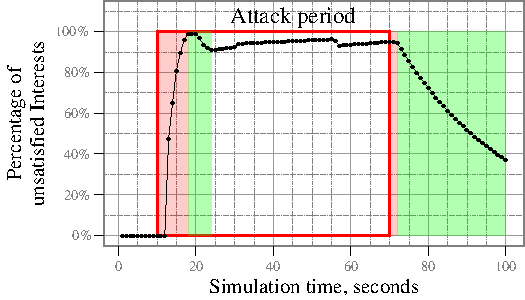
\includegraphics[scale=0.8]{limits}
  \vspace{-0.3cm}
  \caption{Dynamics of the unsatisfied Interests statistics on gateway's interface towards the attacker}
  \label{fig:ratio example}
\end{figure}

%%%%%%%%%%%%%%%%%%%%%%%
%%%%%%%%%%%%%%%%%%%%%%%
%%%%%%%%%%%%%%%%%%%%%%%

\subsubsection{\textbf{Satisfaction-based Interest acceptance}}
\label{sec:probabilistic}

Having successfully implemented a technique to gather statistics on Interest satisfaction ratios, our next challenge is in using this ratio to penalize malicious Interests. A straightforward method to achieve this enforcement is to use the Interest satisfaction ratio as the direct probability for accepting (forwarding) or rejecting an incoming Interest (see Pseudocode~\ref{alg:probabilistic model}).
%Apart from the Interest satisfaction statistics generation, there is a question how this statistics can be used to actually enforce prioritization and penalizing of Interests.


\floatname{algorithm}{\small Pseudocode}

%%%%%%%%%%%%%%%%%%%%%%%%%%%%%%
%%%%%%%%%%%%%%%%%%%%%%%%%%%%%%
%%%%%%%%%%%%%%%%%%%%%%%%%%%%%%

\begin{algorithm}[h]
\footnotesize
\caption{\small Satisfaction-based Interest acceptance}
\label{alg:probabilistic model}
\begin{algorithmic}[1]
\State{} \Comment{Same init, InData and Timeout functions as in Pseudocode~\ref{alg:queuing}}

\vspace{0.1cm}
\Function{OutInterest}{Interest \textbf{i}, InInterface \textbf{in}, OutInterface \textbf{out}}

    \State{} \Comment{Use uniform probability distribution model $P(X)$}
    \State{} \Comment{$P(X) : \forall x \in [0,1] \Rightarrow P(x) = x$}
    
    \If{$F_{in} > \theta $} \Comment{At least some Interests were forwarded before}
        \State $s \leftarrow (1 - U_{in} / F_{in})$
        \State Drop interest with probability $P(s)$
    \EndIf

    \State{forward the Interest, subjecting to token bucket limits}
\EndFunction

\end{algorithmic}
\end{algorithm}

Parameter $\theta$ on line 5 of the Pseudocode~\ref{alg:probabilistic model} ensures that the probabilistic model is not enforced when the volume of Interests arriving at a particular interface is small. This step is critical to provide an opportunity for legitimate users to regain their share of resources after temporary Data delivery failures.

A drawback of the satisfaction-based Interest acceptance method is that each router on the path makes an independent decision on whether to forward or drop an Interest. 
As a result of these independent decisions,  the probability of legitimate Interests being forwarded decreases rapidly as the number of hops between the content requester and producer grows; worsening the Interest satisfaction statistics and resulting in further drops.
In example on Fig.~\ref{fig:flooding example}, the router A observes 50\% satisfaction rate for \texttt{eth1} and 0\% rate for \texttt{eth0}. 
At the same time, router B observes a 30\% satisfaction rate for its \texttt{eth0} interface.
Next time a legitimate Interest arrives at router A, it has a 50\% chance of being forwarded further, and if forwarded, it has only a $50\% \times 30\% = 15\%$ probability of being forwarded further towards the data producer. With each increasing hop in the network, the probability of being forwarded to the next hop decreases significantly. 
One way to prevent this overreaction and unfair penalization is to ensure that the decision taken at each router on whether to forward or drop the Interest is not independent of the decision taken at preceding routers. An explicit notification such as a gossip protocol between neighboring NDN routers might alleviate the problem, but we leave the design and evaluation of it to future work.
%{\color{red}Alex: we should state that it is out of scope of the paper to evaluate this issue}

%%%%%%%%%%%%%%%%%%%%%%%
%%%%%%%%%%%%%%%%%%%%%%%
%%%%%%%%%%%%%%%%%%%%%%%

\subsubsection{\textbf{Satisfaction-based pushback}}
\label{sec:dynamic limits}

% Differential treatment of Interests received from different interfaces can be achieved in a more elegant way, without reverting to probabilistic methods.

The previous algorithm---the satisfaction-based Interest acceptance---divides the available forwarding tokens among all interfaces in proportion to their Interest satisfaction ratios.
% Given the drawbacks of this algorithm, the same effect can be achieved without relying on probabilistic models. 
An alternate algorithm for proportional token distribution without overreaction is to enable and enforce explicit Interest limit for each incoming interface, where the value of the limit depends directly on the interface's Interest satisfaction ratio.
Routers need to announce these limits to their downstream neighbors, ensuring that any Interest forwarded from the downstream router is allowed to get through, resulting in genuine Interest satisfaction statistics.

The formal definition of the satisfaction-based pushback algorithm is presented in Pseudocode~\ref{alg:dynamic limits}, while Fig.~\ref{fig:dynamic limits example} illustrates how the algorithm will work in our example in Fig.~\ref{fig:flooding example}.
Assuming an initial token bucket limit $L=10$ and the current satisfaction ratio for router A is 50\% for \texttt{eth1} and 0\% for \texttt{eth0}, and for router B the ratio is 30\% for \texttt{eth0}, each node will set and announce the following  incoming interface limit $L'$: 
\begin{enumerate}
\item router B will set and announce the incoming interface limit $L'=3$;
\item router A, after receiving announcement from B will readjust its incoming interface limits to $L'_{eth1} = 1.5$ and $L'_{eth0} = 0$; and
\item both legitimate users and adversaries may either obey or ignore the announced limit, which will be in any case enforced by router A.
\end{enumerate}


\begin{figure}[htbp]
  \centering
  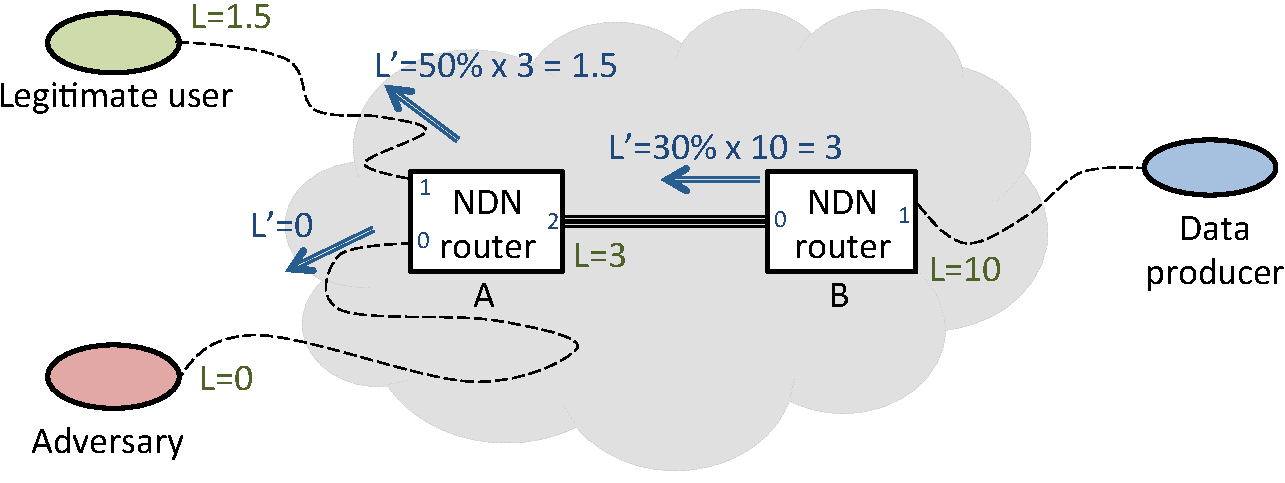
\includegraphics[scale=0.3]{dynamic-limits}
  \vspace{-0.3cm}
  \caption{Satisfaction-based pushback example
%: routers explicitly tell neighbors how many Interest packets they can deliver to the Data producer%
}
  \label{fig:dynamic limits example}
\end{figure}


\floatname{algorithm}{\small Pseudocode}

%%%%%%%%%%%%%%%%%%%%%%%%%%%%%%
%%%%%%%%%%%%%%%%%%%%%%%%%%%%%%
%%%%%%%%%%%%%%%%%%%%%%%%%%%%%%
{ 
\begin{algorithm}[h]
\footnotesize
\caption{\small Satisfaction-based pushback}
\label{alg:dynamic limits}
\begin{algorithmic}[1]
% \State{}\Comment{Same initialization, InData and Timeout functions as in Pseudocode~\ref{alg:queuing}}
\State{} \Comment{Same init, InData and Timeout functions as in Pseudocode~\ref{alg:queuing}}
\vspace{0.1cm}
\State{$\forall f \in \mathrm{interfaces} : L'_{f} \leftarrow L_{f}$} \Comment{Per-incoming interface Interest limit} 

\vspace{0.1cm}

\State{} \Comment{\textit{Announcement from the neighbor}}
\Function{InLimits}{InInterface $in$, Limit $L'$}
    \State $L_{in} \leftarrow L'$
\EndFunction

\vspace{0.1cm}

\Function{AnnounceLimits}{} \Comment{\textit{E.g., every second}}
\For{\textbf{each} outgoing interface $out$}

   \For{\textbf{each} incoming interface $in$}
        \State $L'_{in}= {L_{out}} \times (1 - U_{in}/F_{in})$
        \State AnnounceLimit($in$, $L'_{in}$)
   \EndFor

\EndFor
\EndFunction

\end{algorithmic}
\end{algorithm}


The zero limit for the adversary's link implies that  router A is temporarily not willing to accept any Interests from this interface until the statistics decay to the appropriate level (recall Fig.~\ref{fig:ratio example}).
At the next iteration of the satisfaction-based pushback algorithm, the legitimate user will be able to gradually improve the statistics on both routers A and B as all Interests from the user will get through and return Data, eventually resulting in a full allowance ($L'=L=10$) in the links between the routers A and B, and the user and router A.

We note that while in the description of the satisfaction-based pushback algorithm we explicitly used ``outgoing'' and ``incoming'' interfaces,  all interfaces can be both incoming and outgoing.
Thus, it may not be entirely clear which outgoing limit $L_{out}$ (line 10 in the algorithm) should be used to calculate the incoming limit $L_{in}$.
To overcome this problem, in our actual implementation we enforced separate incoming/outgoing interface limits for each individual FIB entry.
That is, for each FIB entry we set a separate Interest limit for each incoming interface (${L'}_{in}^{fib}$) based on a sum of FIB entry limits for each outgoing interface $L=\sum{L_{out}^{fib}}$.


Both satisfaction-based Interest acceptance and satisfaction-based pushback algorithms are forms of a well-known push-back mechanism~\cite{Pushback}, but with several core differences. 
First, we are suppressing (pushing back) unwanted requests for data, not actual data itself.
Second, differentiating between good and bad Interests is based on the traffic symmetry principle of NDN.
% Alex: I'm not entirely sure about this point... 
Finally, both intelligent attack mitigation algorithms can be deployed at all times without degrading network performance even when there are no active attackers. 

%%% Local Variables: 
%%% mode: latex
%%% TeX-master: "paper"
%%% End: 






\section{Evaluation of Interest flooding mitigation methods}
\label{sec:evaluation}

\todo{Both simulation, as well as emulation for various sized topologies (trees as well as real topologies), various parameters etc.
List all possible parameters, say clearly which ones we vary, and which ones we do not, along with explanations.

Metrics that we will consider in our evaluation (Satisfaction rate for good clients, Link utilization near producers, Latency for good clients, good versus bad interests as a function of time).}

We want to explore the effectiveness of designed mitigation techniques in a two distinctive ways. First, we need to understand how each method works on a very ground level of a just few nodes and links. Second, we want to pick promising techniques and see if they work in a large scale networks of hundreds and thousands of nodes. To ensure the correct transition from small scale experiments to large scale experiments we had to use the same evaluation tool in order to eliminate any possibility of implementation discrepancy. As of today the only network simulator supporting full NDN logic is the NS-3 based ndnSIM software. 

\subsection{Small-scale evaluations}
\label{sec:small-scale}

\begin{figure}[htbp]
  \centering
  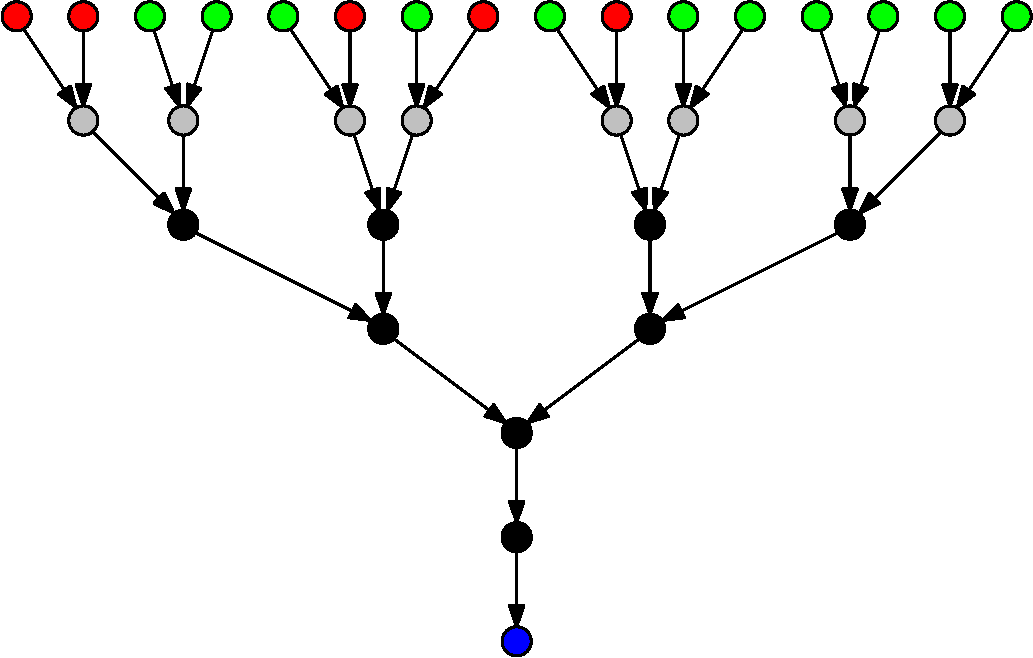
\includegraphics[scale=0.3]{topo-tree-evil-5-good-0-producer-gw}
  \caption{Small-scale topology (one of the runs with 30\% of attackers, all links are 10Mbps with randomized delay 1-10ms)}
  \label{fig:small-scale-topo}
\end{figure}


\begin{figure}[htbp]
  \centering
  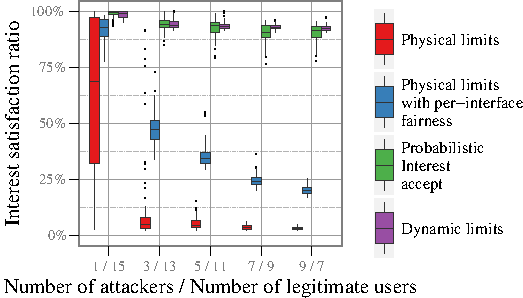
\includegraphics[scale=1]{tree-topo-var-evils-max-consumers-30mins/tree-good-0-producer-gw-avg-1-min}
  \caption{Average consumer Interest satisfaction ratios (first minute)}
  \label{fig:small-scale-topo 1}
\end{figure}


\begin{figure}[htbp]
  \centering
  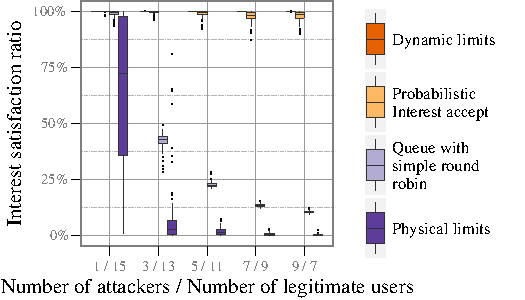
\includegraphics[scale=1]{tree-topo-var-evils-max-consumers-30mins/tree-good-0-producer-gw-avg-1-min-after-1-min}
  \caption{Average consumer Interest satisfaction ratios (second minute)}
  \label{fig:small-scale-topo 2}
\end{figure}

\begin{figure}[htbp]
  \centering
  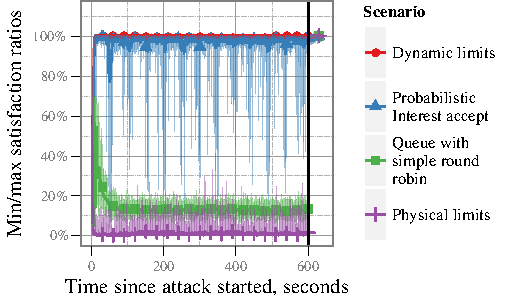
\includegraphics[scale=1]{tree-topo-var-evils-max-consumers-30mins/tree-good-0-producer-gw-dynamics-40}
  \caption{Satisfaction ratio dynamics during the attack (7 attackers / 9 legitimate)}
  \label{fig:small-scale-topo 3}
\end{figure}


%%% Local Variables: 
%%% mode: latex
%%% TeX-master: "paper"
%%% End: 

\subsection{Large scale simulations}
\label{sec:largescale}

Large scale, large scale

%\begin{figure}[htpb]
%  \centering
%  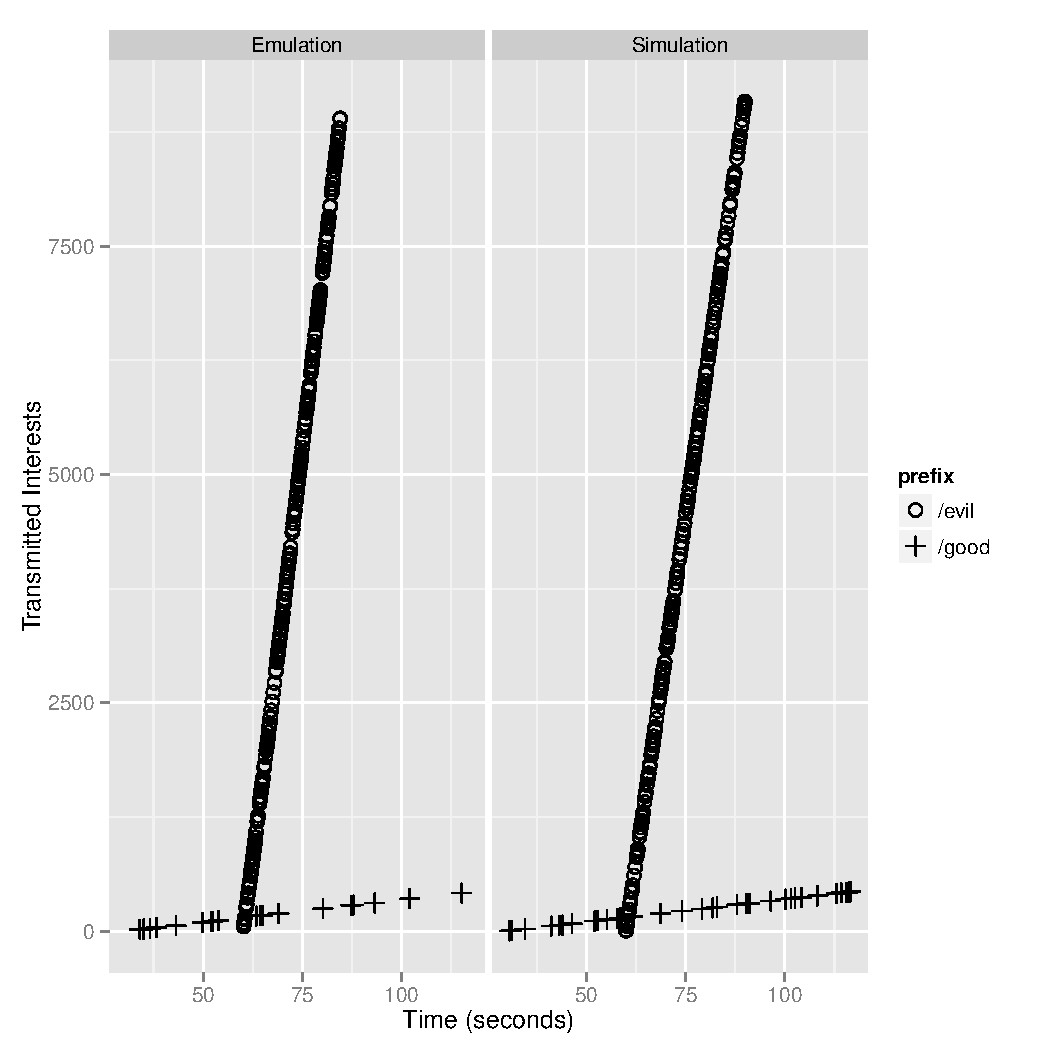
\includegraphics[scale=0.5]{figures/sim-emu-power.pdf}
%  \caption{Strength of Interest flooding attack}
%  \label{fig:simemupower}
%\end{figure}

%\begin{figure}[htpb]
%  \centering
%  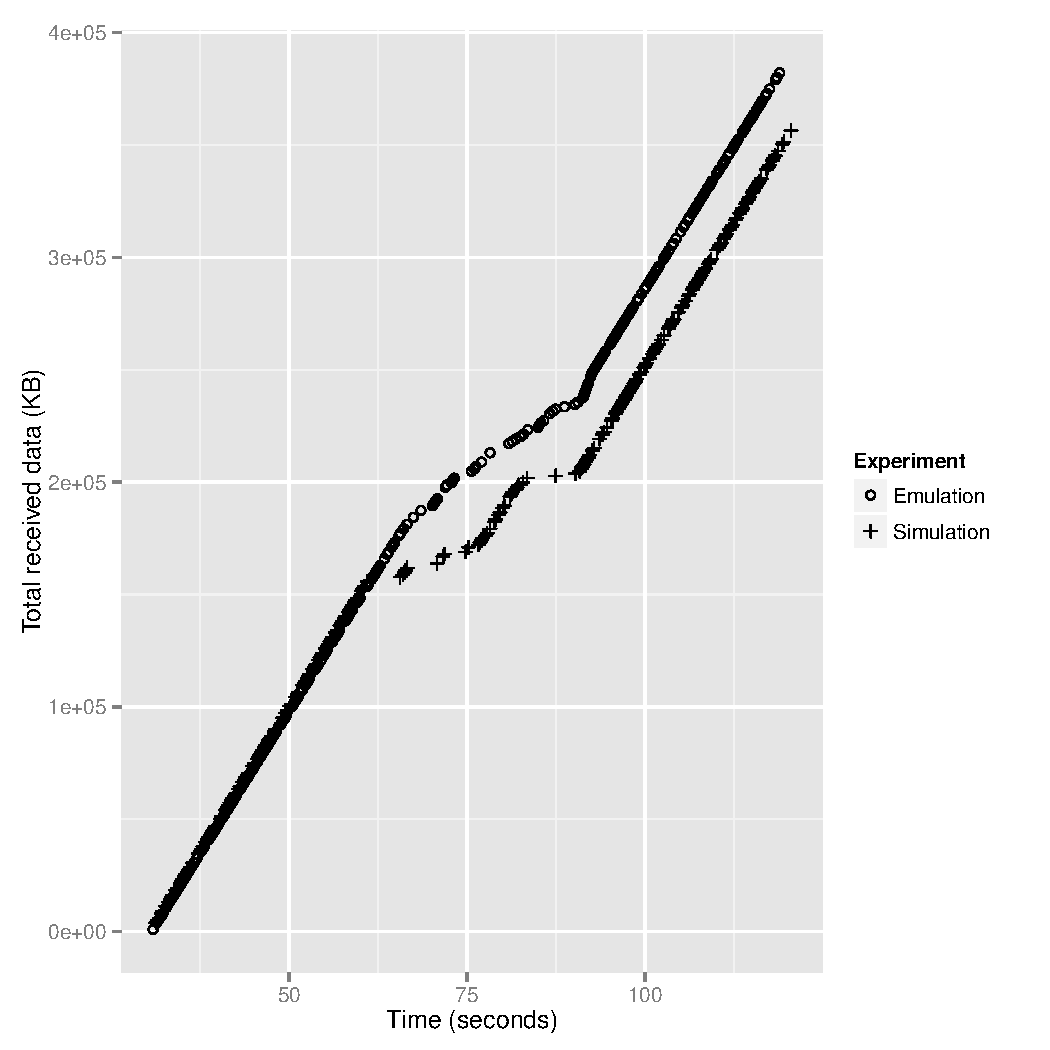
\includegraphics[scale=0.5]{figures/sim-emu-performance.pdf}
%  \caption{Data retrieval by legitimate clients}
%  \label{fig:simemuperf}
%\end{figure}



% \subsection{Simulation versus Emulation}
\label{sec:simemu}
Before committing significant efforts into simulation-based implementation of designed defensive techniques it was necessary to confirm that ndnSIM has close performance characteristics to the reference NDN implementation - Project CCNx. This will guarantee that evaluation results derived from simulations will be meaningful in real NDN world.

To achieve this goal a comparison of Project CCNx software and ndnSIM software was performed under small scale Interest flooding attack. DETER Testbed was used as emulation tool for CCNx evaluation. Using it we were able to setup non-virtualized Ubuntu nodes running CCNx 0.6.0 software connected in a binary tree topology with 4 leaves and 1 root node. A number of applications running on top of CCNx have been developed, namely:
\begin{itemize}
\item{Producer application serves 1KB data packets under a known for the attacker name prefix}
\item{Legitimate client application requests 5KB of data per second from the producer}
\item{Attacker application tries to fill the channel of the producer by sending 500 Interest packets per second}
\end{itemize} 

In this emulation scenario producer application occupied a root node, legitimate clients occupied all even leaves and attacker applications were put on all odd leaves. With 100kb links with 40ms delay such setup leads to no congestion during the period when attackers are turned off and congestion when they are turned on (seconds 60-90). Exactly the same scenario was replicated for ndnSIM evaluation, however, we had to adjust the sending rate of attacker application in order to produce the same amount of congestion in the network. Sending rates are compared in Figure~\ref{fig:simemupower}. To achieve the identical slope and height of sending rate of evil Interests by attacker nodes we had to reduce sending rate of simulation-based attacker application by 30\%. The most likely reason for that is the overhead of Java virtual machine and operating system itself during the emulation of CCNx that results in eventual 30\% slower Interest transmission.  

Once we achieved the same characteristics of Interest flooding attack we were able to compare data packet losses by legitimate clients. Figure~\ref{fig:simemuperf} shows the cumulative received data by legitimate consumers in emulation and simulation experiments. NdnSIM performs worse due to its more deterministic nature, while the effects of UDP protocol usage, operating system process scheduling, and other kernel level operations on packet queues provide more randomness and a better intermixing of bad and good traffic which gives a slightly better performance. To summarize, we can use ndnSIM for our evaluations and real world performance is likely to be even better than our evaluation results.

\begin{figure}[htpb]
  \centering
  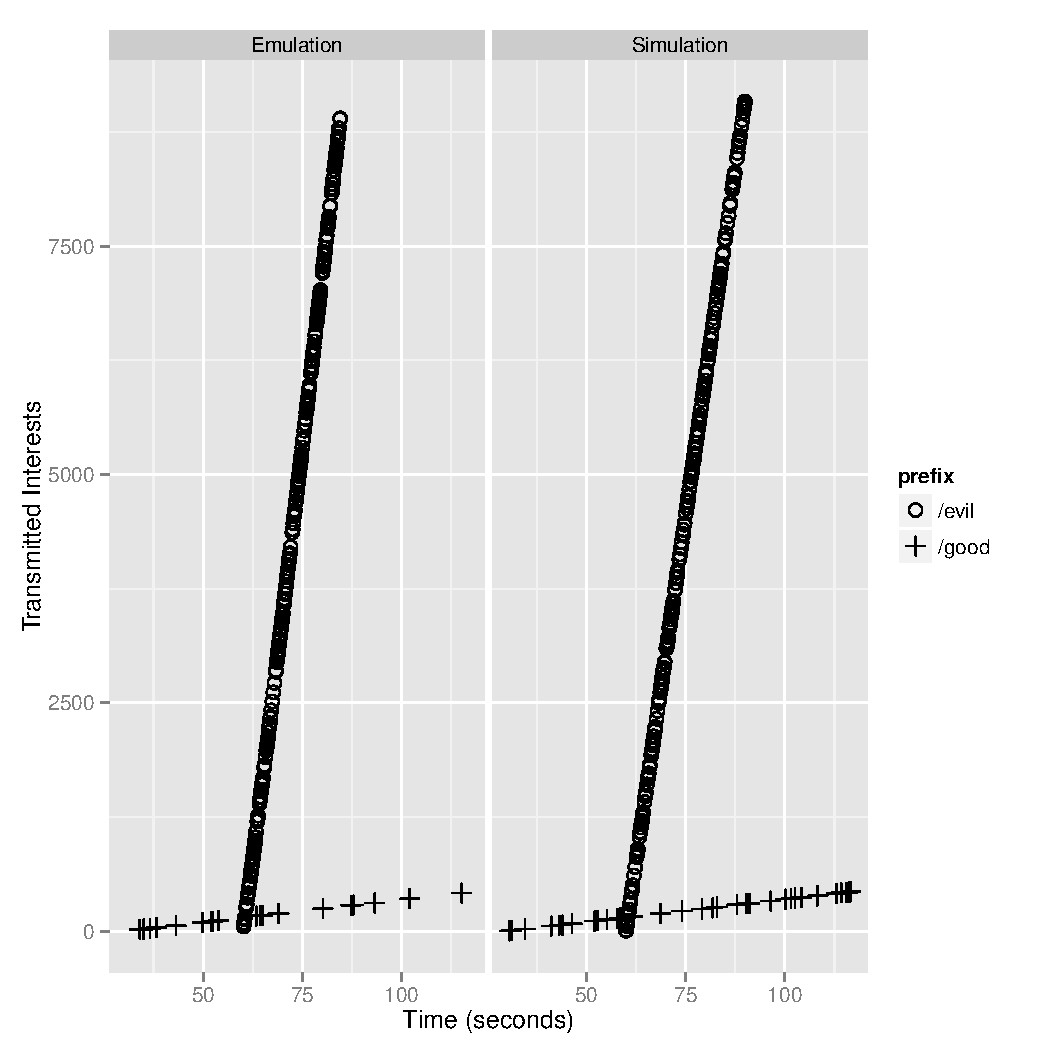
\includegraphics[scale=0.5]{figures/sim-emu-power.pdf}
  \caption{Strength of Interest flooding attack}
  \label{fig:simemupower}
\end{figure}

\begin{figure}[htpb]
  \centering
  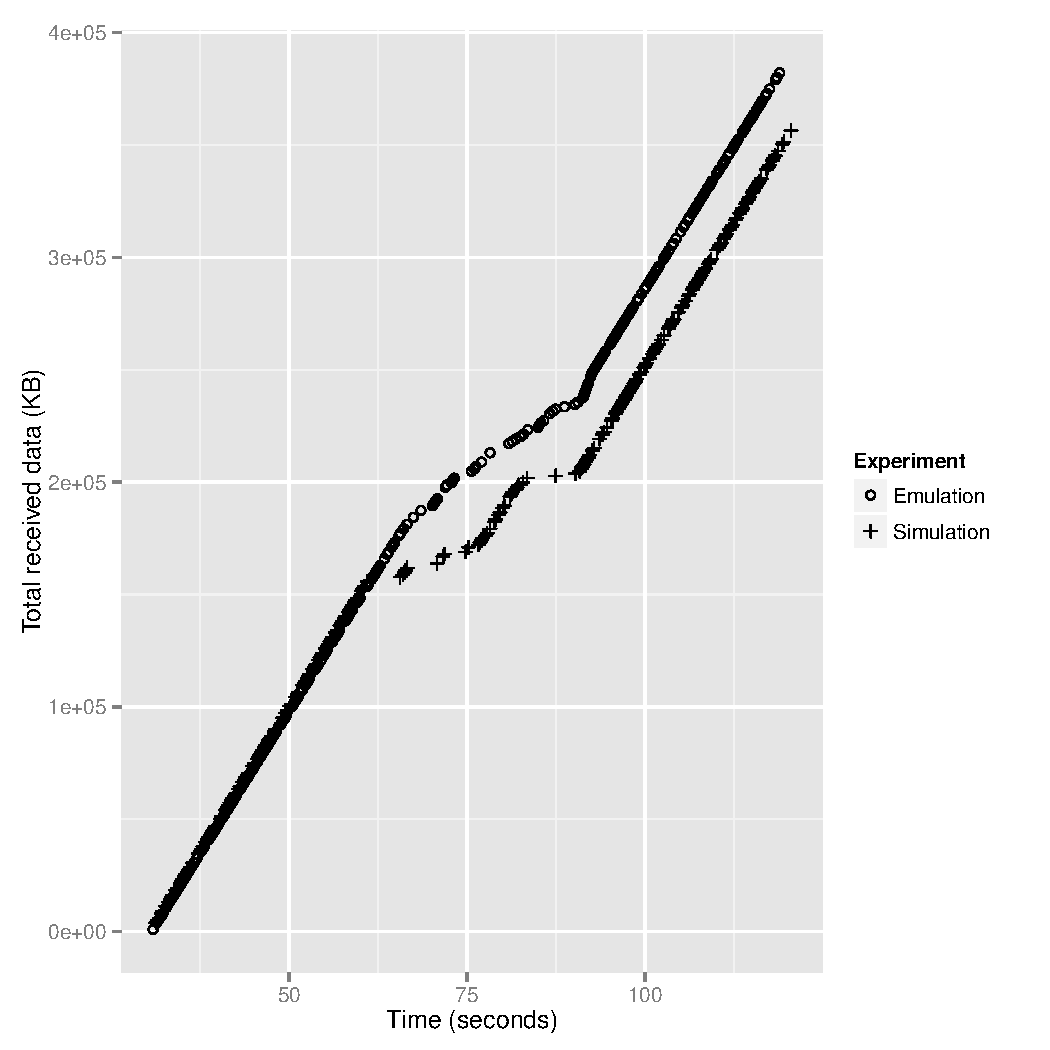
\includegraphics[scale=0.5]{figures/sim-emu-performance.pdf}
  \caption{Data retrieval by legitimate clients}
  \label{fig:simemuperf}
\end{figure}




\section{Related work \label{related-section}}
In this section we provide a classification of mitigation techniques against DDoS flooding attacks in IP networks, because of the lack of any in NDN or other information centric architectures. 
\begin{itemize}
\item{Capability-based systems} allow routers to negotiate, perform and enforce limitations on bandwidth consumption on router-to-router and router-to-client links. Usually such systems require an extensive trust infrastructure in order to validate secure keys used by routers and clients. This implies that each client must pass through an authentication process prior to using any bandwidth ~\cite{Capabilities}.   
\item{Computation-based systems} provide each client an access to the network resources only after performing a significant computations such as solving puzzles. Spending a huge amounts of computational resources can effectively slow down a flooding attack by the botnet, however it also creates additional computational burden for legitimate clients ~\cite{Portcullis}.
\item{Push back systems} are trying to detect bad and good traffic flows on each router, and once attack is detected by one of the routers, it starts a coordinated push back by downrating incoming flows with a bad traffic in order to provide more capacity for a good traffic. This process is reiterating downstream till it reaches edge routers, which are directly connected to attacking bot machines ~\cite{Pushback}. 
\item{Congestion control systems} do per flow traffic analysis and drop of packets belonging to misbehaving flows. For instance, Random Early Detect (RED)~\cite{RED} identifies flows that do not comply with TCP-friendly end-to-end congestion control, and preferentially drop them. If largely deployed such techniques could perform well, however, they cannot provide effective defense against non-greedy botnets that are creating a huge amount of low-bandwidth flows. 
\end{itemize}

%%% Local Variables: 
%%% mode: latex
%%% TeX-master: "paper"
%%% End: 


\section{Discussion}
\label{sec:discussion}

Lessons we learnt, comparison of different mitigation techniques. 
Adapting these to mitigate other DDoS attacks.



\section{Conclusion}
\label{sec:conclusion}

% Main take out from the paper:  could be a problem, but problem is solvable.  

% one may think that 


One of the key components in the Named Data Networking architecture is its stateful data delivery model, which potentially can be abused by new types of denial of service attacks.
However, one should not forget that the same stateful data delivery provides effective mechanisms to fight back against such attacks.
In this paper we demonstrated that NDN architecture can be quite resilient against Interest flooding attacks, which aim to overwhelm network capacity as well as memory resources on NDN routers.
The most effective of the designed algorithms---dynamic limits---almost completely eliminates the attack (or at least mitigates it to an acceptable ``fair'' level), leveraging two key aspects: Interest/Data pah symmetry and full receiver-based traffic control.
In particular, it measures how well Interests are getting satisfied (path symmetry) and uses these measurements to adjust how many Intersets can be accepted from each individual interface (receiver-based control), effectively pushing the attack to the edges.

% Alex: I feel that we should say something else in the conclusion, but not sure what...

% In conclusion, we want to emphasize that Named Data Networking architecture has much more potential, even to protect against attacks,


% We hope that this paper will change attitude to NDN design
% We hope that insights of NDN design potential will 
% Change thinking 
% will spark change in thinking about NDN architecture... 


%%% Local Variables: 
%%% mode: latex
%%% TeX-master: "paper"
%%% End: 



\bibliographystyle{plain}
\bibliography{references}

\end{document}
